% --- Start of Appendix Code ---
\begin{appendices}

  \chapter{Mathematical Reference} % Chapter for definitions and notation
  \label{app:math_reference} % Keep new chapter label

  \section{Glossary of Notation}
  \label{app:math_notation} % Original section label kept

  This section provides a reference for the mathematical notation used throughout this thesis. \ai{Mathematical formulas used here have been generated by AI.}

  \begingroup % Keep longtable formatting local
  \begin{longtable}{p{0.28\textwidth}p{0.68\textwidth}}
    \caption[Summary of Mathematical Notation]{Mathematical Notation} \label{tab:math_notation}                                        \\ % Original table label restored
    % --- Table Header ---
    \toprule
    \textbf{Notation}                           & \textbf{Description}                                                                 \\
    \midrule
    \multicolumn{2}{l}{\textbf{Basic Notation}}                                                                                        \\
    \midrule
    \endfirsthead
    % Header that appears on subsequent pages
    \multicolumn{2}{c}{\tablename\ \thetable{} -- continued from previous page}                                                        \\
    \toprule
    \textbf{Notation}                           & \textbf{Description}                                                                 \\
    \midrule
    \endhead
    % Footer that appears on all pages except the last
    \midrule
    \multicolumn{2}{r}{\textit{Continued on next page}}                                                                                \\
    \endfoot
    % Footer that appears on the last page
    \bottomrule
    \caption*{Source: Author's tabulation.}
    \endlastfoot

    % --- Table Content Starts Here (Identical to original) ---
    $\bm{x}$, $\bm{y}$, $\bm{z}$                & Bold lowercase letters denote vectors                                                \\
    $W$, $A$, $Q$                               & Uppercase letters denote matrices                                                    \\
    $x_i$ or $(\bm{x})_i$                       & Subscript $i$ denotes the $i$-th element of vector $\bm{x}$                          \\
    $W_{ij}$                                    & Subscripts $i,j$ denote the element at row $i$, column $j$ of matrix $W$             \\
    $\bm{h}_t$                                  & Subscript $t$ typically denotes time step or sequence position                       \\
    $\mathbb{R}^n$                              & $n$-dimensional Euclidean space                                                      \\
    $\hat{y}$                                   & Predicted value (in contrast to true value $y$)                                      \\
    \midrule
    \multicolumn{2}{l}{\textbf{Mathematical Operations}}                                                                               \\
    \midrule
    $\odot$                                     & Hadamard (element-wise) product                                                      \\
    $[\bm{a};\bm{b}]$                           & Vertical concatenation of vectors $\bm{a}$ and $\bm{b}$                              \\
    $||\bm{x}||_p$                              & $L_p$ norm of vector $\bm{x}$                                                        \\
    $\nabla J(\theta)$                          & Gradient of function $J$ with respect to parameters $\theta$                         \\
    $d_{\text{Euclidean}}(\bm{a},\bm{b})$       & Euclidean distance between vectors $\bm{a}$ and $\bm{b}$                             \\
    $\text{CosineSimilarity}(\bm{a},\bm{b})$    & Cosine similarity between vectors $\bm{a}$ and $\bm{b}$                              \\
    \midrule
    \multicolumn{2}{l}{\textbf{Neural Network Components}}                                                                             \\
    \midrule
    $\sigma(\cdot)$                             & Sigmoid activation function                                                          \\
    $\tanh(\cdot)$                              & Hyperbolic tangent activation function                                               \\
    $\text{ReLU}(\cdot)$                        & Rectified Linear Unit activation function                                            \\
    $\text{softmax}(\bm{z})$                    & Softmax function applied to vector $\bm{z}$                                          \\
    $\vec{\bm{h}}_t$, $\cev{\bm{h}}_t$          & Forward and backward hidden states in Bi-LSTM                                        \\
    $\bm{h}_{\text{mean\_pool}}$                & Result of mean pooling operation on sequence                                         \\
    $\bm{h}_{\text{max\_pool}}$                 & Result of max pooling operation on sequence                                          \\
    $\bm{\gamma}$, $\bm{\beta}$                 & Scale and shift parameters in normalization layers                                   \\
    \midrule
    \multicolumn{2}{l}{\textbf{Optimization}}                                                                                          \\
    \midrule
    $\eta$                                      & Learning rate in optimization algorithms                                             \\
    $\lambda$                                   & Regularization strength parameter                                                    \\
    $\epsilon$                                  & Small constant added for numerical stability                                         \\
    $\bm{m}_t$, $\bm{v}_t$                      & First and second moment estimates in Adam optimizer                                  \\
    $\hat{\bm{m}}_t$, $\hat{\bm{v}}_t$          & Bias-corrected moment estimates in Adam optimizer                                    \\
    \midrule
    \multicolumn{2}{l}{\textbf{Loss Functions and Performance Metrics}}                                                                \\
    \midrule
    $\text{BCE}$                                & Binary Cross-Entropy loss function                                                   \\
    $\text{MSE}$                                & Mean Squared Error metric                                                            \\
    $\text{MAE}$                                & Mean Absolute Error metric                                                           \\
    $\text{MAPE}$                               & Mean Absolute Percentage Error metric                                                \\
    $\text{Precision}$                          & Precision metric in binary classification                                            \\
    $\text{Recall}$                             & Recall (sensitivity) metric in binary classification                                 \\
    $\text{F1}$                                 & F1-score, harmonic mean of precision and recall                                      \\
    $AUC$                                       & Area Under the Curve metric for binary classification                                \\
    $ROC$                                       & Receiver Operating Characteristic curve                                              \\
    $TPR$, $FPR$                                & True Positive Rate and False Positive Rate                                           \\
    $TP$, $TN$, $FP$, $FN$                      & True Positive, True Negative, False Positive, False Negative counts                  \\
    \midrule
    \multicolumn{2}{l}{\textbf{Statistical Concepts}}                                                                                  \\
    \midrule
    $\mu$, $\sigma^2$                           & Mean and variance of a distribution                                                  \\
    $\mathcal{N}(\mu,\sigma^2)$                 & Normal (Gaussian) distribution with mean $\mu$ and variance $\sigma^2$               \\
    $\text{UCL}$, $\text{LCL}$                  & Upper and Lower Control Limits in statistical process control                        \\
    $p$                                         & Proportion (typically of anomalies) in statistical process control                   \\
    $H_0$                                       & Null hypothesis in statistical testing                                               \\
    $\alpha$                                    & Significance level in statistical testing                                            \\
    $S_{obs}$                                   & Observed test statistic in permutation testing                                       \\
    $N$                                         & Number of permutations in permutation testing                                        \\
    $p$-value                                   & Probability of observing test statistic at least as extreme as $S_{obs}$ under $H_0$ \\
    $RR$                                        & Rejection rate of null hypothesis                                                    \\
    \midrule
    \multicolumn{2}{l}{\textbf{Feature Engineering}}                                                                                   \\
    \midrule
    $x_{\sin}$, $x_{\cos}$                      & Sine and cosine transformations of cyclical feature $x$                              \\
    $P$                                         & Period of cyclical feature in time encoding                                          \\
    $\mathcal{F}_c$                             & Feature subset in feature selection methods                                          \\
    \midrule
    \multicolumn{2}{l}{\textbf{Attention Mechanism}}                                                                                   \\
    \midrule
    $Q$, $K$, $V$                               & Query, Key, and Value matrices in attention mechanism                                \\
    $d_k$                                       & Dimension of key vectors in attention mechanism                                      \\
    \midrule
    \multicolumn{2}{l}{\textbf{Dataset Notation}}                                                                                      \\
    \midrule
    $\mathcal{D}$                               & Dataset or distribution                                                              \\
    $\mathcal{D}_{train}$, $\mathcal{D}_{test}$ & Training and testing datasets                                                        \\
    $\mathcal{D}_{real}$, $\mathcal{D}_{sim}$   & Real-world and simulation datasets                                                   \\
    \midrule
    \multicolumn{2}{l}{\textbf{Statistical Tests and Combinations}}                                                                    \\
    \midrule
    $p_i$                                       & Individual p-value from the $i$-th statistical test                                  \\
    $k$                                         & Number of independent or related tests being combined                                \\
    $t_i$                                       & Cauchy-transformed p-value in the CCT method                                         \\
    $T_{CCT}$                                   & Combined test statistic in the Cauchy Combination Test                               \\
    $P_{CCT}$                                   & Combined p-value from the Cauchy Combination Test                                    \\
    $k_{obs}$                                   & Observed number of rejections across $k$ tests                                       \\
    $P_{Binom}$                                 & P-value from the Binomial test for rejection rates                                   \\
    $B(k, \alpha)$                              & Binomial distribution with $k$ trials and success probability $\alpha$               \\
  \end{longtable}
  \endgroup


  \section{Mathematical and Computational Foundations}
  \label{app:math_foundations} % Original section label kept

  This section provides formal definitions and illustrations for core mathematical and computational concepts used in the thesis, supplementing the main text.

  \subsection{Basic Vector and Matrix Operations}
  \label{subsec:basic_ops_app} % New label for this subsection
  As established in \autoref{app:math_notation}, vectors are denoted by bold lowercase letters (e.g., \( \bm{z} \)) and matrices by uppercase letters (e.g., \( W \)). Vectors are assumed to be column vectors unless otherwise specified.

  \paragraph{Matrix-Vector Multiplication:}
  Given a matrix \( W \in \mathbb{R}^{m \times n} \) and a vector \( \bm{x} \in \mathbb{R}^n \), their product is a vector \( \bm{y} = W\bm{x} \in \mathbb{R}^m \), where the \( i \)-th element is calculated as:
  \begin{equation}
    y_i = \sum_{j=1}^{n} W_{ij} x_j % No original label
  \end{equation}

  \paragraph{Vector Addition:}
  Given two vectors \( \bm{y}, \bm{b} \in \mathbb{R}^m \), their sum is a vector \( \bm{z} = \bm{y} + \bm{b} \in \mathbb{R}^m \), computed element-wise:
  \begin{equation}
    z_i = y_i + b_i % No original label
  \end{equation}

  \paragraph{Element-wise (Hadamard) Product:}
  Given two vectors \( \bm{a}, \bm{b} \in \mathbb{R}^m \), their Hadamard product is a vector \( \bm{c} = \bm{a} \odot \bm{b} \in \mathbb{R}^m \), computed element-wise:
  \begin{equation}
    c_i = a_i \cdot b_i % No original label
  \end{equation}
  This operation is notably used in LSTM cells (see main text, e.g., \autoref{sec:lstm}). % Reference kept

  \paragraph{Vector Concatenation:}
  Given two vectors \( \bm{a} \in \mathbb{R}^{d_a} \) and \( \bm{b} \in \mathbb{R}^{d_b} \), their concatenation \( \bm{c} = [\bm{a} ; \bm{b}] \) results in a vector \( \bm{c} \in \mathbb{R}^{d_a + d_b} \) formed by stacking the elements of \( \bm{b} \) below the elements of \( \bm{a} \). This is used in Bi-LSTMs and Multi-Head Attention (see main text, e.g., Eq.~\ref{eq:bilstm_concat} and Eq.~\ref{eq:multihead_attention}). % References kept

  \paragraph{Matrix Transpose:}
  The transpose of a matrix \( A \in \mathbb{R}^{m \times n} \), denoted \( A^T \in \mathbb{R}^{n \times m} \), is obtained by swapping its rows and columns:
  \begin{equation}
    (A^T)_{ij} = A_{ji} % No original label
  \end{equation}
  This is used in the Scaled Dot-Product Attention formula (see main text, e.g., Eq.~\ref{eq:scaled_dot_product_attention}). % Reference kept

  \subsection{Activation Functions}
  \label{subsec:activations_app} % New label for this subsection
  Activation functions introduce non-linearity into neural network models, allowing them to learn complex patterns. They are typically applied element-wise to the output of a linear transformation \( \bm{z} = W\bm{x} + \bm{b} \).

  \paragraph{Sigmoid Function (\( \sigma \)):}
  The standard sigmoid function maps any real input to the range (0, 1). It is defined as:
  \begin{equation}
    \sigma(z) = \frac{1}{1 + e^{-z}} % No original label
  \end{equation}
  Due to its output range, it is commonly used for gating mechanisms in LSTMs (see main text, e.g., Equations~\ref{eq:lstm-forget-gate}, \ref{eq:lstm-input-gate}, \ref{eq:lstm-output-gate}) and for producing probabilities in binary classification outputs. A plot is shown in Figure~\ref{fig:sigmoid_plot}.

  \begin{figure}[htbp] % Use htbp or other specifiers instead of H if possible
    \centering
    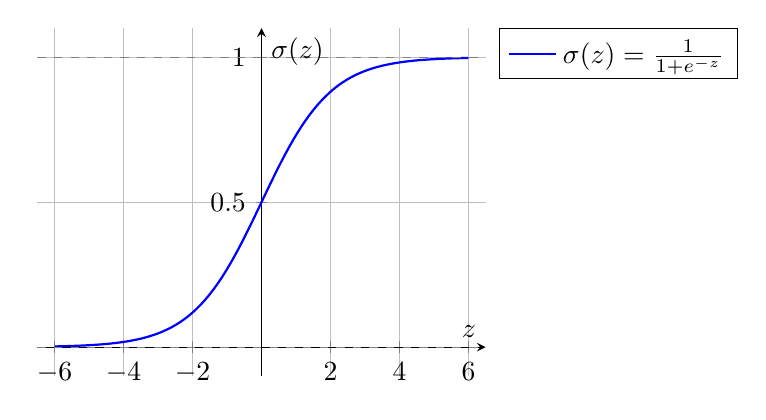
\begin{tikzpicture}
      \begin{axis}[
          width=0.6\textwidth, % Adjust width as needed
          height=6cm,
          axis lines=middle,
          xlabel={$z$},
          ylabel={$\sigma(z)$},
          grid=major,
          ymin=-0.1, ymax=1.1,
          xmin=-6.5, xmax=6.5,
          samples=100,
          domain=-6:6,
          legend pos=outer north east % Or other position
        ]
        \addplot [blue, thick] {1/(1+exp(-x))};
        \addlegendentry{$\sigma(z) = \frac{1}{1+e^{-z}}$}
        % Asymptotes
        \addplot [dashed, gray, domain=-6.5:6.5] {0};
        \addplot [dashed, gray, domain=-6.5:6.5] {1};
      \end{axis}
    \end{tikzpicture}
    \caption[Sigmoid Activation Function]{The Sigmoid activation function.}
    \label{fig:sigmoid_plot} % Original figure label restored
    \caption*{Author's illustration.}
  \end{figure}


  \paragraph{Hyperbolic Tangent Function (\( \tanh \)):}
  The hyperbolic tangent function maps any real input to the range (-1, 1). It is defined as:
  \begin{equation}
    \tanh(z) = \frac{e^z - e^{-z}}{e^z + e^{-z}} = 2\sigma(2z) - 1 % No original label
  \end{equation}
  It is frequently used as the main activation function for hidden states in RNNs and LSTMs (see main text, e.g., Equations~\ref{eq:rnn_hidden_state}, \ref{eq:lstm-candidate-cell}, \ref{eq:lstm-hidden-state}). See Figure~\ref{fig:tanh_plot}.

  \begin{figure}[htbp]
    \centering
    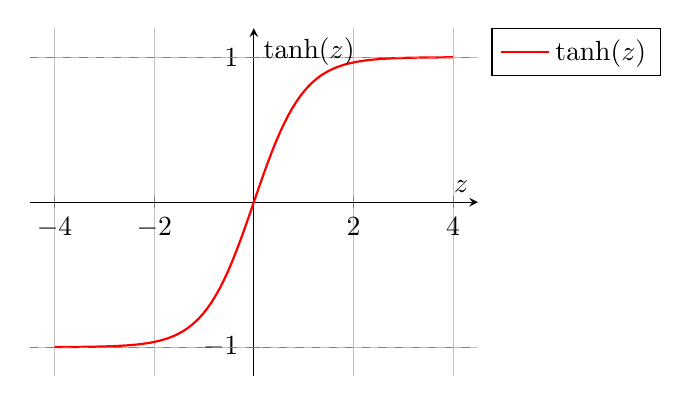
\begin{tikzpicture}
      \begin{axis}[
          width=0.6\textwidth,
          height=6cm,
          axis lines=middle,
          xlabel={$z$},
          ylabel={$\tanh(z)$},
          grid=major,
          ymin=-1.2, ymax=1.2,
          xmin=-4.5, xmax=4.5,
          samples=100,
          domain=-4:4,
          legend pos=outer north east
        ]
        \addplot [red, thick] {tanh(x)};
        \addlegendentry{$\tanh(z)$}
        % Asymptotes
        \addplot [dashed, gray, domain=-4.5:4.5] {-1};
        \addplot [dashed, gray, domain=-4.5:4.5] {1};
      \end{axis}
    \end{tikzpicture}
    \caption[Tanh activation function]{The Hyperbolic Tangent (tanh) activation function.}
    \label{fig:tanh_plot} % Original figure label restored
    \caption*{Author's illustration.}
  \end{figure}


  \paragraph{Rectified Linear Unit (ReLU):}
  The ReLU function outputs the input directly if it is positive, and zero otherwise. It is defined as:
  \begin{equation}
    \text{ReLU}(z) = \max(0, z) % No original label
  \end{equation}
  ReLU is widely used in deep learning due to its simplicity and effectiveness in mitigating the vanishing gradient problem for positive inputs. It is used within the model presented in this thesis (see main text, e.g., Section~\ref{sec:integrated_architecture}). See Figure~\ref{fig:relu_plot}.

  \begin{figure}[htbp]
    \centering
    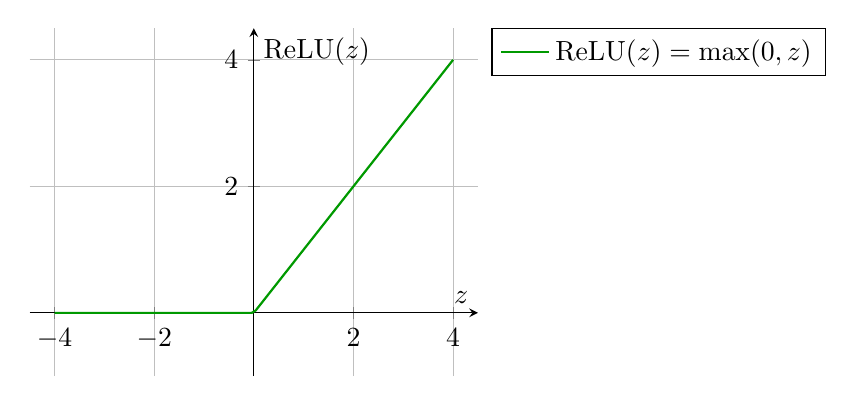
\begin{tikzpicture}
      \begin{axis}[
          width=0.6\textwidth,
          height=6cm,
          axis lines=middle,
          xlabel={$z$},
          ylabel={ReLU$(z)$},
          grid=major,
          ymin=-1, ymax=4.5,
          xmin=-4.5, xmax=4.5,
          samples=100,
          legend pos=outer north east
        ]
        \addplot [green!60!black, thick, domain=-4:4] {max(0,x)};
        \addlegendentry{ReLU$(z) = \max(0, z)$}
      \end{axis}
    \end{tikzpicture}
    \caption[ReLU activation function]{The Rectified Linear Unit (ReLU) activation function.}
    \label{fig:relu_plot} % Original figure label restored
    \caption*{Author's illustration.}
  \end{figure}


  \paragraph{Softmax Function:}
  The softmax function converts a vector of K real numbers \( \bm{z} = (z_1, ..., z_K) \) into a probability distribution consisting of K probabilities. The function is applied to the entire vector and the \( i \)-th element of the output vector is calculated as:
  \begin{equation}
    \text{softmax}(\bm{z})_i = \frac{e^{z_i}}{\sum_{j=1}^K e^{z_j}} \quad \text{for } i = 1, ..., K % No original label
  \end{equation}
  The outputs are non-negative and sum to 1 (\( \sum_{i=1}^K \text{softmax}(\bm{z})_i = 1 \)). Softmax is commonly used in the output layer of multi-class classification models and plays a crucial role in normalizing scores into attention weights in the Attention mechanism (see main text, e.g., Equation~\ref{eq:scaled_dot_product_attention}).

  \subsection{Distance and Similarity Metrics}
  \label{subsec:distance_metrics} % Original subsection label kept
  These metrics quantify the difference or similarity between vectors, which is fundamental in many machine learning tasks. Let \( \bm{a}, \bm{b} \in \mathbb{R}^d \) be two vectors of dimension \( d \).

  \paragraph{Euclidean Distance (L2 Distance):}
  \label{eq:euclidean_distance} % Original equation label restored
  The most common distance measure:
  \begin{equation}
    d_{\text{Euclidean}}(\bm{a}, \bm{b}) = ||\bm{a} - \bm{b}||_2 = \sqrt{\sum_{i=1}^d (a_i - b_i)^2}
  \end{equation}

  \paragraph{Manhattan Distance (L1 Distance):}
  Measures distance along axes at right angles:
  \begin{equation}
    d_{\text{Manhattan}}(\bm{a}, \bm{b}) = ||\bm{a} - \bm{b}||_1 = \sum_{i=1}^d |a_i - b_i| % No original label
  \end{equation}

  \paragraph{Cosine Similarity:}
  Measures the cosine of the angle between vectors:
  \begin{equation}
    \text{CosineSimilarity}(\bm{a}, \bm{b}) = \frac{\bm{a} \cdot \bm{b}}{||\bm{a}||_2 ||\bm{b}||_2} = \frac{\sum_{i=1}^d a_i b_i}{\sqrt{\sum_{i=1}^d a_i^2} \sqrt{\sum_{i=1}^d b_i^2}} % No original label
  \end{equation}
  Widely used for high-dimensional vectors. Cosine Distance is sometimes defined as \( 1 - \text{CosineSimilarity}(\bm{a}, \bm{b}) \).

  \subsection{Neural Network Techniques}
  \label{subsec:nn_techniques_app} % New label for this subsection

  \paragraph{Attention Mechanism Components:}
  The Scaled Dot-Product Attention mechanism relies on:
  \begin{itemize}
    \item \textit{Dot Product Similarity:} Compatibility between query \( \bm{q} \) and key \( \bm{k} \) often computed as \( \bm{q}^T \bm{k} \). Matrix product \( QK^T \) computes pairwise dot products.
    \item \textit{Scaling:} Scores \( QK^T \) are divided by \( \sqrt{d_k} \) before softmax to stabilize gradients, especially for large \( d_k \).
  \end{itemize}

  \paragraph{Normalization Techniques:}
  Help stabilize training and improve convergence.
  \begin{itemize}
    \item \textit{Layer Normalization (LayerNorm):} Normalizes inputs across features for \textit{each individual data sample}. Computation is independent of batch size. For input vector \( \bm{x} \):
          \begin{equation}
            \text{LayerNorm}(\bm{x}) = \bm{\gamma} \odot \frac{\bm{x} - \mu_{\text{sample}}}{\sqrt{\sigma^2_{\text{sample}} + \epsilon}} + \bm{\beta}
            \label{eq:layernorm} % Original equation label restored
          \end{equation}
          \( \mu_{\text{sample}} \), \( \sigma^2_{\text{sample}} \) are mean/variance across features of \( \bm{x} \). \( \bm{\gamma}, \bm{\beta} \) are learnable scale/shift parameters. Frequently used in RNNs and Transformers (used in this thesis).
    \item \textit{Batch Normalization (BatchNorm):} (Included for contrast) Normalizes across the \textit{batch dimension} for each feature. Effective in CNNs, but dependence on batch statistics can be less suitable for sequence models.
  \end{itemize}

  \paragraph{Pooling Strategies for Sequences:}
  Aggregate information across the sequence dimension \( H = [\bm{h}_1, \bm{h}_2, ..., \bm{h}_T] \), where \( \bm{h}_t \in \mathbb{R}^d \).
  \begin{itemize}
    \item \textit{Mean Pooling:} Calculates element-wise average:
          \begin{equation}
            \bm{h}_{\text{mean\_pool}} = \frac{1}{T} \sum_{t=1}^T \bm{h}_t % No original label
          \end{equation}
          Result \( \bm{h}_{\text{mean\_pool}} \in \mathbb{R}^d \) represents average activation. Used in this thesis.
    \item \textit{Max Pooling:} Calculates element-wise maximum:
          \begin{equation}
            (\bm{h}_{\text{max\_pool}})_j = \max_{t=1...T} (\bm{h}_t)_j \quad \text{for } j = 1, ..., d % No original label
          \end{equation}
          Result \( \bm{h}_{\text{max\_pool}} \in \mathbb{R}^d \) captures strongest activation per feature.
  \end{itemize}

  \paragraph{Weight Initialization:} Crucial for effective training.
  \begin{itemize}
    \item \textit{Kaiming (He) Initialization:} For ReLU layers \autocite{he2015delving}. Aims to keep variance constant. Kaiming Normal init draws weights from \( \mathcal{N}(0, \text{std}^2) \) with:
          \begin{equation}
            \text{std} = \sqrt{\frac{2}{\text{fan\_in}}} % No original label
          \end{equation}
          `fan\_in` is the number of input units. Used in this thesis.
    \item \textit{Xavier (Glorot) Initialization:} For symmetric activations (tanh, sigmoid) \autocite{glorot2010understanding}. Aims to keep variance constant across layers. Xavier Normal init uses:
          \begin{equation}
            \text{std} = \sqrt{\frac{2}{\text{fan\_in} + \text{fan\_out}}} % No original label
          \end{equation}
          `fan\_out` is the number of output units.
  \end{itemize}

  \paragraph{Regularization Techniques:} Prevent overfitting.
  \begin{itemize}
    \item \textit{L2 Regularization (Weight Decay):} Adds penalty to loss function proportional to squared magnitude of weights \( \theta \):
          \begin{equation}
            J_{reg}(\theta) = J(\theta) + \frac{\lambda}{2} ||\theta||_2^2 = J(\theta) + \frac{\lambda}{2} \sum_i \theta_i^2 % No original label
          \end{equation}
          \( \lambda \) is regularization strength. Encourages smaller weights.
    \item \textit{Dropout:} Randomly sets a fraction of neuron activations to zero during training \autocite{srivastava2014dropout}. Prevents co-adaptation. Dropout rate specifies the zeroing probability. Used in this thesis (LSTM layers and fully connected block).
  \end{itemize}

  \paragraph{Data Handling for Sequences:}
  \begin{itemize}
    \item \textit{Sequence Padding:} Augments shorter sequences in a batch with padding values (often zero) to match the longest sequence, creating uniform tensors. `collate_fn` in this thesis uses `pad_sequence`. Important to mask padded values in subsequent computations (loss, attention).
  \end{itemize}


  \subsection{Optimization Algorithms}
  \label{subsec:optimization_app} % New label for this subsection
  Update model parameters \( \theta \) to minimize loss \( J(\theta) \).

  \paragraph{Stochastic Gradient Descent (SGD):}
  Fundamental algorithm updating parameters based on mini-batch gradient:
  \begin{equation}
    \theta_{k+1} = \theta_k - \eta \nabla J(\theta_k; \bm{x}^{(i)}; \bm{y}^{(i)}) % No original label
  \end{equation}
  \( \eta \) is learning rate. Variants include momentum.

  \paragraph{Adam Optimizer:}
  % Note: Original text referred to \label{eq:adam} in text, but labelled the equation eq:adam-update.
  % Keep the equation label as eq:adam-update. If \ref{eq:adam} was used elsewhere, it needs fixing.
  Adaptive learning rate algorithm using first and second moment estimates of gradients \autocite{kingma2014adam}. Computes biased moments (\( \bm{m}_t, \bm{v}_t \)), bias-corrected moments (\( \hat{\bm{m}}_t, \hat{\bm{v}}_t \)), and updates:
  \begin{equation}
    \theta_{t+1} = \theta_t - \frac{\eta}{\sqrt{\hat{\bm{v}}_t} + \epsilon} \hat{\bm{m}}_t
    \label{eq:adam-update} % Original equation label restored
  \end{equation}
  Used for training the model in this work.

  \paragraph{Learning Rate Scheduling:}
  Adjust \( \eta \) during training to improve convergence.
  \begin{itemize}
    \item \textit{ReduceLROnPlateau:} Reduces \( \eta \) if a monitored metric (e.g., validation loss) stops improving for 'patience' epochs. Employed in this thesis.
    \item \textit{Step Decay:} Reduces \( \eta \) by fixed factor every N epochs.
    \item \textit{Cosine Annealing:} Decreases \( \eta \) following a cosine curve.
  \end{itemize}

  \subsection{Loss Functions and Metrics}
  \label{subsec:loss_metrics_app} % New label for this subsection
  Quantify the difference between predictions and true values.

  \paragraph{Binary Cross-Entropy (BCE):}
  \label{eq:bce} % Original equation label restored
  For binary classification tasks ($y_i \in \{0, 1\}$, prediction $\hat{p}_i$). Loss function used in this thesis.
  \begin{equation}
    \text{BCE} = -\frac{1}{N} \sum_{i=1}^N [ y_i \log(\hat{p}_i) + (1 - y_i) \log(1 - \hat{p}_i) ]
  \end{equation}

  \paragraph{Regression Metrics:}
  For evaluating models predicting continuous variables.
  \begin{itemize}
    \item \textit{Mean Squared Error (MSE):} Average of squared differences. Sensitive to outliers \autocite{fahrmeir2016statistik}.
          \begin{equation}
            \text{MSE} = \frac{1}{n} \sum_{i=1}^{n} (y_i - \hat{y}_i)^2 % No original label
          \end{equation}
    \item \textit{Mean Absolute Error (MAE):} Average of absolute differences. More robust to outliers \autocite{fahrmeir2016statistik}.
          \begin{equation}
            \text{MAE} = \frac{1}{n} \sum_{i=1}^{n} |y_i - \hat{y}_i| % No original label
          \end{equation}
    \item \textit{Mean Absolute Percentage Error (MAPE):} Average percentage difference. Useful when scale varies.
          \begin{equation}
            \text{MAPE} = \frac{1}{n} \sum_{i=1}^{n} \left| \frac{y_i - \hat{y}_i}{y_i} \right| \times 100\% % No original label
          \end{equation}
  \end{itemize}


  \subsection{Decision Tree Splitting Criteria}
  \label{subsec:decision_tree_splitting_criteria} % Original subsection label kept

  \paragraph{Gini Impurity}
  Measures the probability of incorrect classification if a randomly chosen sample from the node were randomly labeled according to the class distribution at the node. For $K$ classes ($K = 2$ here), with $p_k$ being the proportion of samples of class $k$ in set $S$:
  \begin{equation}
    G(S) = 1 - \sum_{k=1}^{K} p_k^2
    \label{eq:gini_impurity} % Original equation label restored
  \end{equation}
  A lower Gini impurity indicates a purer node. Split quality (dividing $S$ into $S_{left}$, $S_{right}$) is evaluated by weighted average impurity:
  \begin{equation}
    \text{Gini}_{\text{split}}(S) = \frac{|S_{left}|}{|S|} G(S_{left}) + \frac{|S_{right}|}{|S|} G(S_{right})
    \label{eq:gini_split} % Original equation label restored
  \end{equation}
  The DTree seeks splits that minimize this value \autocite{breiman1984classification}.


  \chapter{Statistical Validation Methodology} % Chapter for detailed stat methods
  \label{app:cct} % Original chapter label kept (was app:cct, makes sense here)

  This chapter details the statistical tests used for combining results across multiple runs and assessing overall significance, complementing the permutation testing described in the main text (e.g., \autoref{sec:permtest}).

  \section{Cauchy Combination Test (CCT)}
  \label{sec:cct_methodology} % Original section label kept

  The Cauchy Combination Test \autocite{liu2020cauchy} provides a powerful method for combining $k$ individual p-values, $p_1, p_2, ..., p_k$, obtained from multiple statistical tests (in this case, the $k=10$ runs of the permutation test for each feature subset) into a single overall p-value. A key advantage of the CCT is its robustness under arbitrary dependence structures among the individual p-values.

  The CCT transforms each individual p-value $p_i$ using the inverse CDF of the standard Cauchy distribution ($C(0,1)$), equivalent to using the tangent function:
  \begin{equation}
    t_i = \tan\left( (0.5 - p_i) \pi \right)
    \label{eq:cct_transform} % Original equation label restored
  \end{equation}
  The combined test statistic, $T_{CCT}$, is the mean (assuming equal weights $w_i=1/k$) of these transformed values:
  \begin{equation}
    T_{CCT} = \frac{1}{k} \sum_{i=1}^k t_i = \frac{1}{k} \sum_{i=1}^k \tan\left( (0.5 - p_i) \pi \right)
    \label{eq:cct_statistic} % Original equation label restored
  \end{equation}
  Under the global null hypothesis, $T_{CCT}$ approximately follows a standard Cauchy distribution, $C(0,1)$.

  The final combined p-value, $P_{CCT}$, is the upper tail probability:
  \begin{equation}
    P_{CCT} = P(C(0,1) \ge T_{CCT}) = 1 - F_{C(0,1)}(T_{CCT}) = 0.5 - \frac{\arctan(T_{CCT})}{\pi}
    \label{eq:cct_pvalue} % Original equation label restored
  \end{equation}
  where $F_{C(0,1)}$ is the CDF of the standard Cauchy distribution. A small $P_{CCT}$ indicates strong evidence against the global null. The CCT is powerful when the signal is sparse and robust to dependence.

  \section{Binomial Test for Rejection Rate}
  \label{sec:binom_test_methodology} % Original section label kept

  The Binomial test formally assesses the significance of the observed \textit{Rejection Rate} ($RR$) \autocite{fahrmeir2016statistik}, defined as the proportion of $k$ runs where the null hypothesis $H_0$ was rejected at significance level $\alpha$. $RR = k_{obs}/k$, where $k_{obs}$ is the observed number of rejections ($p_{run} < \alpha$).

  The test addresses: "Is $k_{obs}$ significantly greater than expected by chance if $H_0$ were true for all runs?"

  The null hypothesis ($H_0$) for the Binomial test is that the true probability of rejecting in a single run is $\alpha$. Under $H_0$, the number of rejections $X$ follows a Binomial distribution:
  \begin{equation}
    X \sim B(k, \alpha) % No original label
  \end{equation}
  The probability mass function (PMF) is:
  \begin{equation}
    P(X=i | k, \alpha) = \binom{k}{i} \alpha^i (1-\alpha)^{k-i}
    \label{eq:binom_pmf} % Original equation label restored
  \end{equation}
  The p-value for observing $k_{obs}$ or more rejections (one-sided test) is:
  \begin{equation}
    P_{Binom} = P(X \ge k_{obs} | H_0) = \sum_{i=k_{obs}}^{k} P(X=i | k, \alpha) = \sum_{i=k_{obs}}^{k} \binom{k}{i} \alpha^i (1-\alpha)^{k-i}
    \label{eq:binom_pvalue} % Original equation label restored
  \end{equation}
  A small $P_{Binom}$ suggests the observed $RR$ is significantly higher than expected by chance. This complements methods like CCT by focusing on the consistency of rejection.


  \chapter{Detailed Validation Results} % Chapter for results tables
  \label{app:detailed_results} % New label for this chapter

  This chapter presents the detailed numerical results from the statistical validation analyses discussed in \autoref{app:cct}. % Reference updated to chapter label

  \section{Decision Tree Model Results}
  \label{sec:dt_results_appendix} % Original section label kept

  The following table presents the detailed hypothesis testing results obtained using the DTree as the model for distinguishing between real and simulated data. The evaluation metric was the ROC AUC score. The results are based on $k=10$ independent runs, each employing $N=1000$ permutations for p-value calculation. The significance level for individual run rejection and the Binomial test was set at $\alpha=0.05$. The Cauchy Combination Test (CCT) was used to combine p-values across runs (yielding $P_{CCT}$), and the Binomial test assessed the significance of the observed Rejection Rate ($RR$, yielding $P_{Binom}$).

  \begin{table}[htbp] % Using htbp allows LaTeX more flexibility in placement
    \centering
    \caption[Detailed Decision Tree Model Results applying CCT]{Detailed Decision Tree validation results across 10 runs (N=1000, $\alpha=0.05$).}
    \label{tab:results-dt-appendix} % Original table label restored
    \resizebox{\textwidth}{!}{%
      \begin{tabular}{l c c c c c p{3cm}}
        \toprule
        \textbf{Component ($\mathcal{F}_c$)} & \textbf{$\overline{\text{ROC AUC}}$} & \textbf{$\sigma_{\text{ROC AUC}}$} & \textbf{$P_{CCT}$} & \textbf{RR} & \textbf{$P_{Binom}$} & \textbf{Assessment} \\
        \midrule
        \texttt{time\_model}                 & 1.0000                               & 0.0000                             & 0.0000             & 1.00        & 0.0000               & INACCURATE          \\
        \texttt{resource\_model}             & 0.9817                               & 0.0088                             & 0.0000             & 1.00        & 0.0000               & INACCURATE          \\
        \texttt{transformation\_model}       & 1.0000                               & 0.0000                             & 0.0000             & 1.00        & 0.0000               & INACCURATE          \\
        \texttt{transition\_model}           & 1.0000                               & 0.0000                             & 0.0000             & 1.00        & 0.0000               & INACCURATE          \\
        \texttt{process\_model}              & 1.0000                               & 0.0000                             & 0.0000             & 1.00        & 0.0000               & INACCURATE          \\
        \texttt{kpi\_based}                  & 1.0000                               & 0.0000                             & 0.0000             & 1.00        & 0.0000               & INACCURATE          \\
        \texttt{all\_features}               & 1.0000                               & 0.0000                             & 0.0000             & 1.00        & 0.0000               & INACCURATE          \\
        \bottomrule
      \end{tabular}%
    }
    \caption*{Source: Author's tabulation based on permutation test results.}
  \end{table}

  As evidenced by the results in Table \ref{tab:results-dt-appendix}, both the Cauchy Combination Test ($P_{CCT}=0.0000$) and the Binomial test ($P_{Binom}=0.0000$) yielded extremely significant p-values for all feature subsets when using the Decision Tree model at $\alpha=0.05$. The perfect rejection rate ($RR=1.00$) across all components further underscores this. This indicates a highly consistent and statistically robust ability of the DT model to distinguish between the real and simulated data across all evaluated components based on the engineered features, leading to the assessment "INACCURATE" for all components according to the defined validation framework.

  \section{BiLSTM Model Results}
  \label{sec:lstm_results_appendix} % Original section label kept

  The following table presents the detailed hypothesis testing results obtained using the BiLSTM classifier as the blackbox model for distinguishing between real and simulated data. The evaluation metric was the ROC AUC score. The results are based on $k=10$ independent runs, each employing $N=1000$ permutations for p-value calculation. The significance level for individual run rejection and the Binomial test was set at $\alpha=0.01$. The Cauchy Combination Test (CCT) was used to combine p-values across runs (yielding $P_{CCT}$), and the Binomial test assessed the significance of the observed Rejection Rate ($RR$, yielding $P_{Binom}$).

  \begin{table}[htbp] % Using htbp allows LaTeX more flexibility in placement
    \centering
    \caption[Detailed BiLSTM Model Results]{Detailed BiLSTM validation results across 10 runs (N=1000, $\alpha=0.01$).}
    \label{tab:results-lstm-appendix} % Original table label restored
    \resizebox{\textwidth}{!}{%
      \begin{tabular}{l l l l l l p{3cm}}
        \toprule
        \textbf{Component ($\mathcal{F}_c$)} & \textbf{$\overline{\text{ROC AUC}}$} & \textbf{$\sigma_{\text{ROC AUC}}$} & \textbf{$P_{CCT}$} & \textbf{RR} & \textbf{$P_{Binom}$} & \textbf{Assessment} \\
        \midrule
        \texttt{time\_model}                 & 1.0000                               & 0.0000                             & 0.0000             & 1.00        & 0.0000               & INACCURATE          \\
        \texttt{resource\_model}             & 0.9945                               & 0.0071                             & 0.0000             & 1.00        & 0.0000               & INACCURATE          \\
        \texttt{transformation\_model}       & 1.0000                               & 0.0000                             & 0.0000             & 1.00        & 0.0000               & INACCURATE          \\
        \texttt{transition\_model}           & 0.9644                               & 0.1067                             & 0.0000             & 1.00        & 0.0000               & INACCURATE          \\
        \texttt{process\_model}              & 0.9714                               & 0.0858                             & 0.0000             & 1.00        & 0.0000               & INACCURATE          \\
        \texttt{kpi\_based}                  & 0.9975                               & 0.0054                             & 0.0000             & 1.00        & 0.0000               & INACCURATE          \\
        \texttt{all\_features}               & 1.0000                               & 0.0000                             & 0.0000             & 1.00        & 0.0000               & INACCURATE          \\
        \bottomrule
      \end{tabular}%
    }
    \caption*{Source: Author's tabulation based on permutation test results.}
  \end{table}

  As shown in Table \ref{tab:results-lstm-appendix}, the results for the BiLSTM model are the same observed with the DTree. Using the stricter significance level of $\alpha=0.01$, both the CCT ($P_{CCT}=0.0000$) and the Binomial test ($P_{Binom}=0.0000$) yielded extremely significant p-values for all feature subsets. The rejection rate was also perfect ($RR=1.00$) across all components. This demonstrates a consistent and statistically robust capability of the BiLSTM model to distinguish between the real and simulated data across all SBDT components evaluated, leading to the assessment "INACCURATE" for all components within the validation framework.


  \chapter{Supplementary Figures} % Chapter for figures not embedded above
  \label{app:supp_figures} % New label for this chapter

  \section{Design Science Research Methodology}
  \label{app:dsr_figure} % New label for this section
  \begin{figure}[htbp] % Use H with caution, consider htbp
    \centering
    % Make sure the path 'figures/dsr.png' is correct relative to your main .tex file
    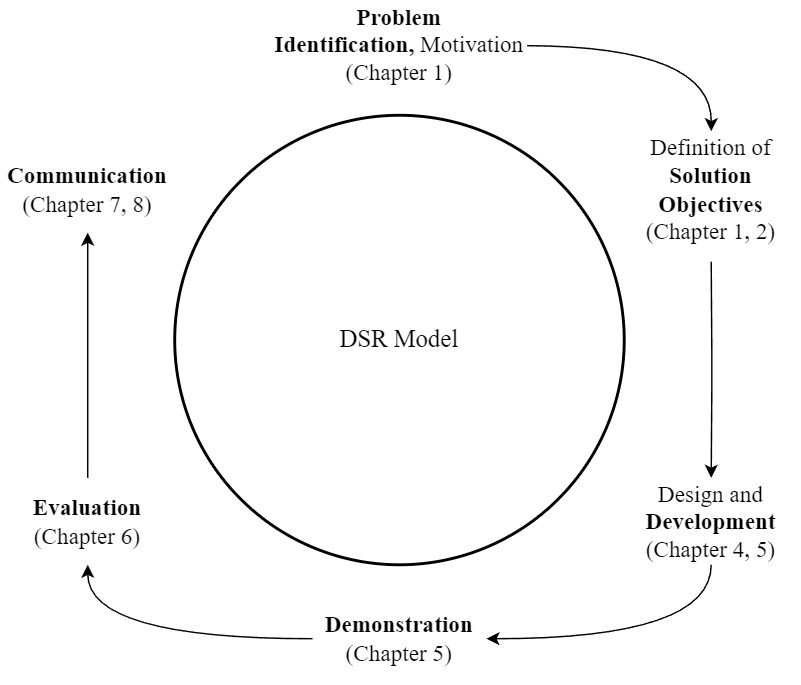
\includegraphics[width=0.6\textwidth]{figures/dsr.png}
    \caption[Design Science Methodology]{The cyclical design science research model. The model consists of six steps. The problem identification (1) refers to the research gap in automated \gls{vvuq} of \gls{sbdt}. Defining the solution objectives (2) specifies the research gap by formulating questions and hypotheses based on the theoretical foundations. The design and development (3) phase includes the development of the framework. The demonstration (4) phase shows the application of the framework in a case study. The evaluation (5) phase assesses the effectiveness of the framework. The communication (6) phase concludes the research by presenting the results.}
    \label{fig:DSR} % Original figure label restored
    \caption*{Illustration based on \textcite{peffers2007design}}
  \end{figure}

  \section{Time Encoding on Unit Circle}
  \label{app:time_encoding_figure} % New label for this section
  % Note: This figure could also be placed within App A, Section "Neural Network Techniques"
  % near Feature Engineering / Time Encoding if preferred.
  \begin{figure}[htbp] % Use H with caution, consider htbp
    \centering
    \begin{tikzpicture}[
        scale=3, % Adjust scale to change overall size
        hour dot/.style={circle, fill=blue!70, inner sep=1.5pt},
        hour label/.style={font=\small}
      ]

      % Draw the unit circle
      \draw [gray, dashed] (0,0) circle (1);

      % Draw axes
      \draw [->, gray!80] (-1.3,0) -- (1.3,0) node[right, black] {$x_{\cos}$};
      \draw [->, gray!80] (0,-1.3) -- (0,1.3) node[above, black] {$x_{\sin}$};
      \node[above=5pt] at (current bounding box.north) {Hour of Day Encoded on Unit Circle}; % Title


      % Plot hour points and labels
      \foreach \h in {0,...,23} {
          % Calculate angle in degrees (TikZ trigonometric functions use degrees)
          \pgfmathsetmacro{\angle}{\h * 360 / 24}

          % Draw the point for the hour
          \node[hour dot] at (\angle:1) {}; % Place dot using polar coordinates (angle:radius)

          % Add labels for key hours slightly outside the circle
          \ifnum \h = 0 \node[hour label, anchor=west] at (\angle:1.15) {0h (Midnight)}; \fi
          \ifnum \h = 3 \node[hour label, anchor=south west] at (\angle:1.15) {3h}; \fi
          \ifnum \h = 6 \node[hour label, anchor=south] at (\angle:1.15) {6h (Morning)}; \fi
          \ifnum \h = 9 \node[hour label, anchor=south east] at (\angle:1.15) {9h}; \fi
          \ifnum \h = 12 \node[hour label, anchor=east] at (\angle:1.15) {12h (Noon)}; \fi
          \ifnum \h = 15 \node[hour label, anchor=north east] at (\angle:1.15) {15h}; \fi
          \ifnum \h = 18 \node[hour label, anchor=north] at (\angle:1.15) {18h (Evening)}; \fi
          \ifnum \h = 21 \node[hour label, anchor=north west] at (\angle:1.15) {21h}; \fi
        }

    \end{tikzpicture}
    \caption[Feature Transformation]{Sine and Cosine transformation of the hour of the day (0-23). Each hour is mapped to a point $(x_{\cos}, x_{\sin})$ on the unit circle (blue dots). Key hours are labelled, demonstrating how the transformation preserves cyclical continuity (hour 23 is near hour 0).}
    \label{fig:time-encoding} % Original figure label restored
    \caption*{Source: Author's illustration}
  \end{figure}

\end{appendices}
% --- End of Appendix Code ---